%yright 2007, 2008, 2009 Elsevier Ltd
%% 
%% This file is part of the 'Elsarticle Bundle'.
%% ---------------------------------------------
%% 
%% It may be distributed under the conditions of the LaTeX Project Public
%% License, either version 1.2 of this license or (at your option) any
%% later version.  The latest version of this license is in
%%    http://www.latex-project.org/lppl.txt
%% and version 1.2 or later is part of all distributions of LaTeX
%% version 1999/12/01 or later.
%% 
%% The list of all files belonging to the 'Elsarticle Bundle' is
%% given in the file `manifest.txt'.
%% 

%% Template article for Elsevier's document class `elsarticle'
%% with numbered style bibliographic references
%% SP 2008/03/01

% \documentclass[preprint,11pt]{elsarticle}
\documentclass[final,1p,11pt]{elsarticle}

%\documentclass[final,1p,times]{elsarticle}


%% Use the option review to obtain double line spacing
%%\documentclass[authoryear,preprint,review,12pt]{elsarticle}

%% Use the options 1p,twocolumn; 3p; 3p,twocolumn; 5p; or 5p,twocolumn
%% for a journal layout:
%% \documentclass[final,1p,times]{elsarticle}
%% \documentclass[final,1p,times,twocolumn]{elsarticle}
%% \documentclass[final,3p,times]{elsarticle}
%% \documentclass[final,3p,times,twocolumn]{elsarticle}
%% \documentclass[final,5p,times]{elsarticle}
%% \documentclass[final,5p,times,twocolumn]{elsarticle}

%%% For including figures, graphicx.sty has been loaded in
%% elsarticle.cls. If you prefer to use the old commands
%% please give \usepackage{epsfig}


\usepackage{epsfig}
%\usepackage{cite}
%\usepackage{mcite}
\usepackage{array,tabularx,epsfig,mathrsfs,graphicx,rotating}
\usepackage{ifthen}
\usepackage{amsfonts}
\usepackage{ragged2e}
\PassOptionsToPackage{hyphens}{url}
\usepackage[hyphens]{url}
\usepackage{hyperref}
\usepackage{listings}
\usepackage{subfigure}
\usepackage{epstopdf}
% Custom colors
\usepackage{color}
\usepackage{float}

% to cross text
\usepackage[normalem]{ulem} % either use this (simple) or
\usepackage{soul} % use this (many fancier options)


\hypersetup{
  colorlinks=true,
  linkcolor=blue,
  citecolor=blue,
  urlcolor=blue
}




\graphicspath{{figs/}}


\pdfinfo{
   /Author (Chekanov/Demarteau)
   /Title  (Conceptual Design Studies for a CEPC Detector)
   /CreationDate (D:20160102195600)
   /Subject (PDFLaTeX)
   /Keywords (PDF;LaTeX)
}


\textheight=22cm
\textwidth=14.5cm

\newcommand{\beq}{\begin{equation}}
\newcommand{\eeq}{\end{equation}}
\newcommand{\la}{\langle}
\newcommand{\promc}{{\sc ProMC}}
\newcommand{\ra}{\rangle}
\newcommand{\eps}{\epsilon}
\newcommand{\ud}{\mathrm{d}}
\newcommand{\Ec}{\mathcal{E}}
\newcommand{\Fc}{\mathcal{F}}
\newcommand{\Za}{\mathrm{Z_1}}
\newcommand{\Zb}{\mathrm{Z_2}}
\newcommand{\Zn}{\mathrm{Z_n}}
\newcommand{\F}{\mathrm{F}}

\chardef\til=126
\newcommand{\mev}{{\,\mathrm{MeV}}}
\newcommand{\gev}{{\,\mathrm{GeV}}}
\newcommand{\tev}{{\,\mathrm{TeV}}}
\newcommand{\GEANTfour} {\textsc{geant4}}
\journal{XXX-XXX}



\begin{document}
%50bins
\begin{figure}
\begin{center}
   \subfigure[40TeV at 20$\times$20(cm$\times$cm) in cluster ( no cut )] {
   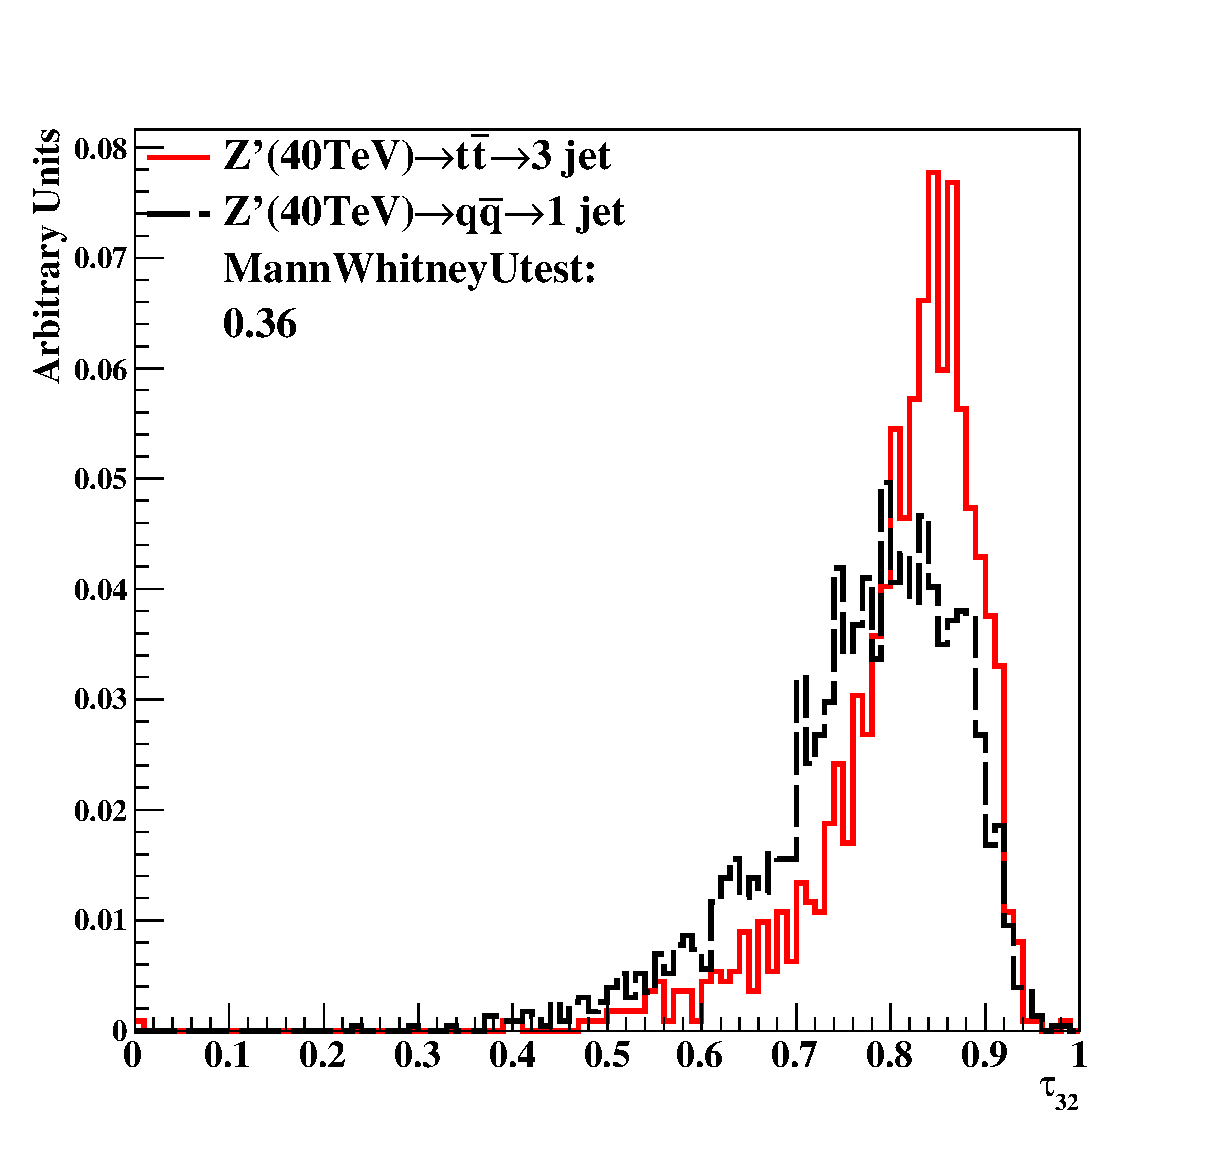
\includegraphics[width=0.43\textwidth]{figs/Dis_cluster_010_tau32_40tev_04_no_cut_Man_100.eps}
   }
      \subfigure[40TeV at 20$\times$20(cm$\times$cm) in cluster (after cut)] {
   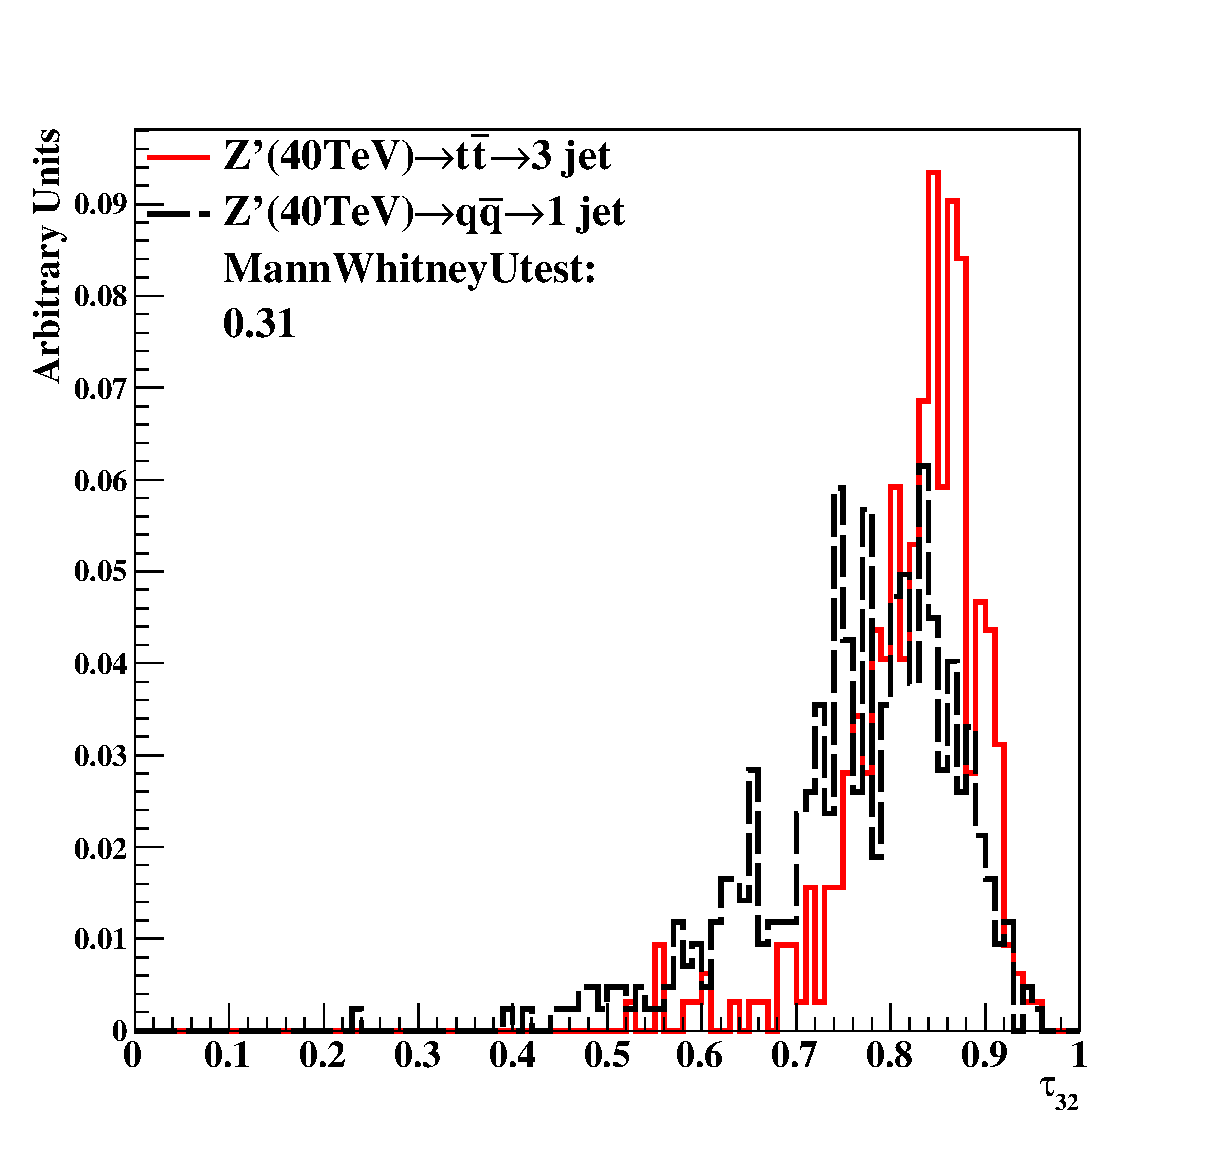
\includegraphics[width=0.43\textwidth]{figs/Dis_cluster_010_tau32_40tev_04_after_cut_Man_100.eps}
   }
   \subfigure[40TeV at 5$\times$5(cm$\times$cm) in cluster ( no cut )] {
   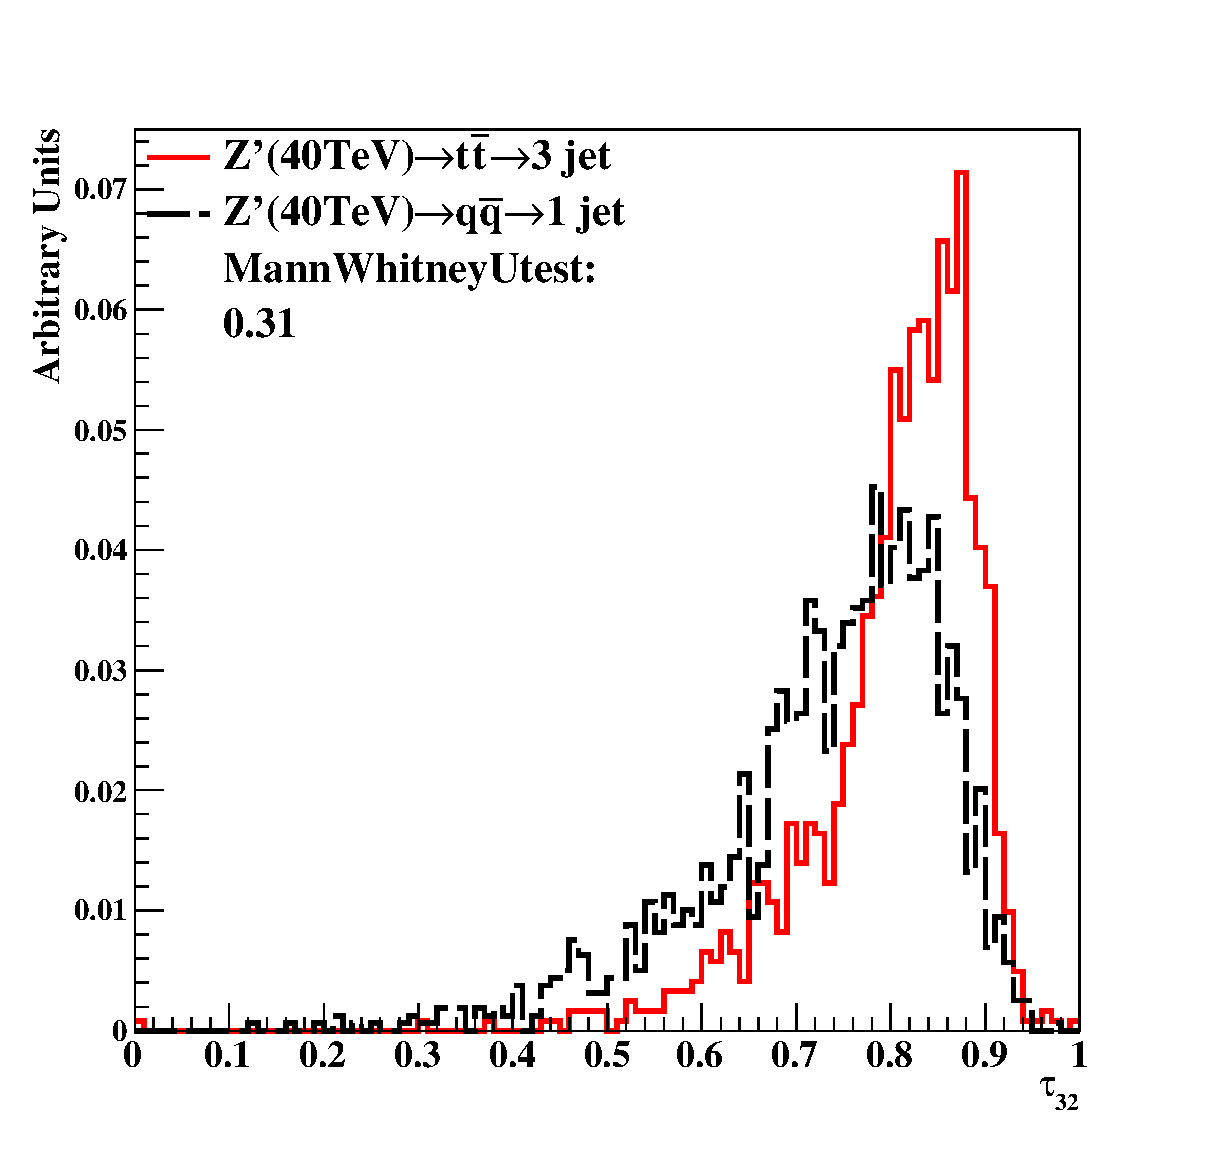
\includegraphics[width=0.43\textwidth]{figs/Dis_cluster_009_tau32_40tev_04_no_cut_Man_100.eps}
   }
    \subfigure[40TeV at 5$\times$5(cm$\times$cm) in cluster ( after cut )] {
   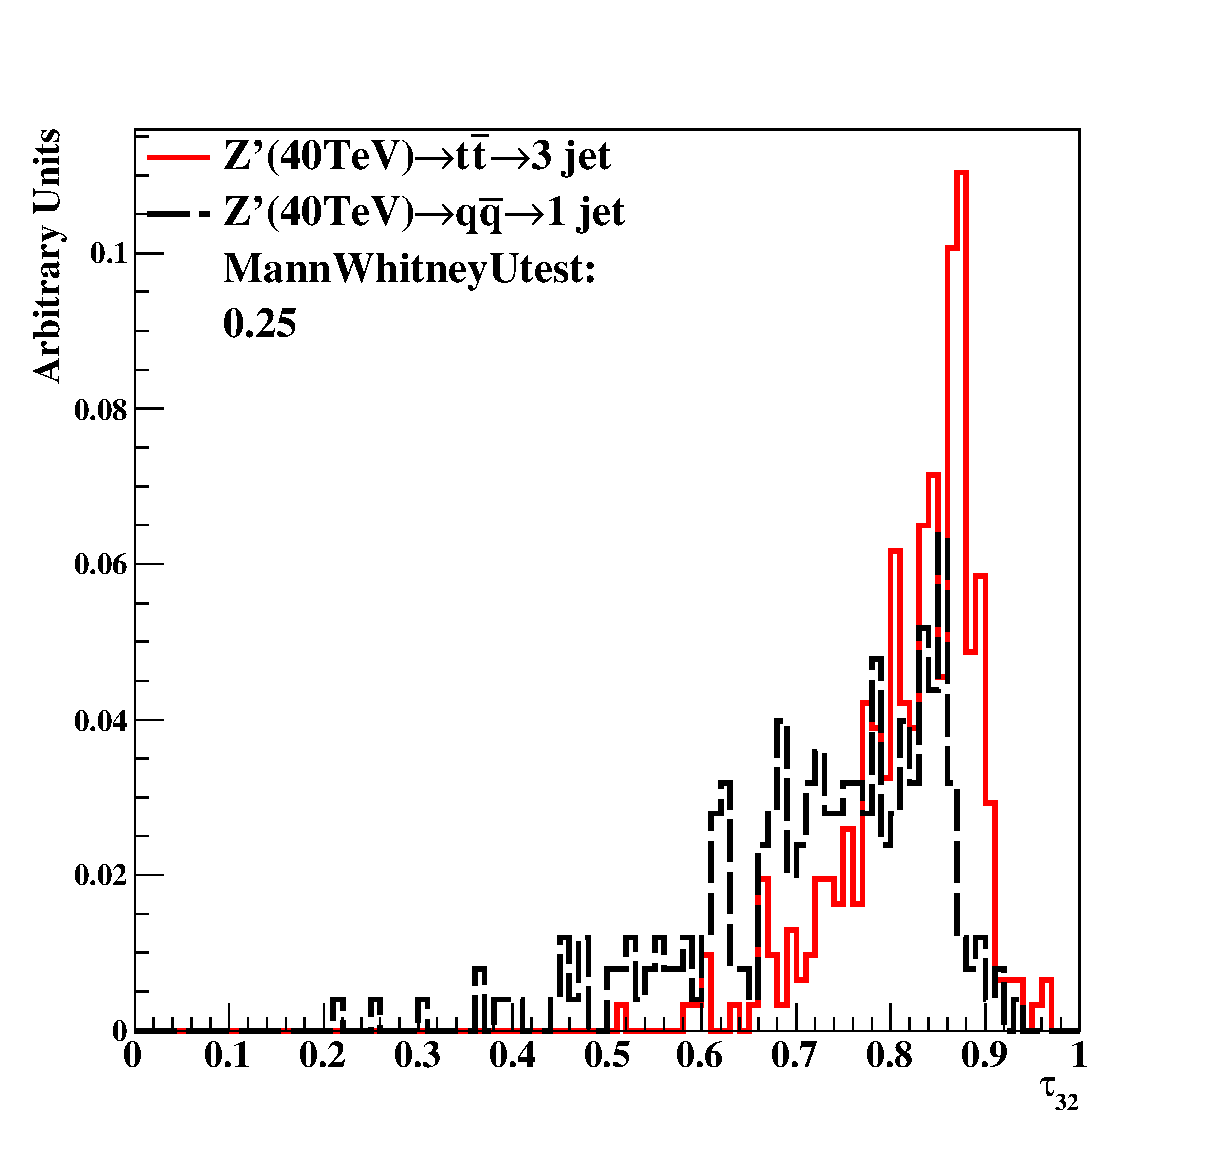
\includegraphics[width=0.43\textwidth]{figs/Dis_cluster_009_tau32_40tev_04_after_cut_Man_100.eps}
   }
   \subfigure[40TeV at 1$\times$1(cm$\times$cm) in cluster ( no cut )] {
   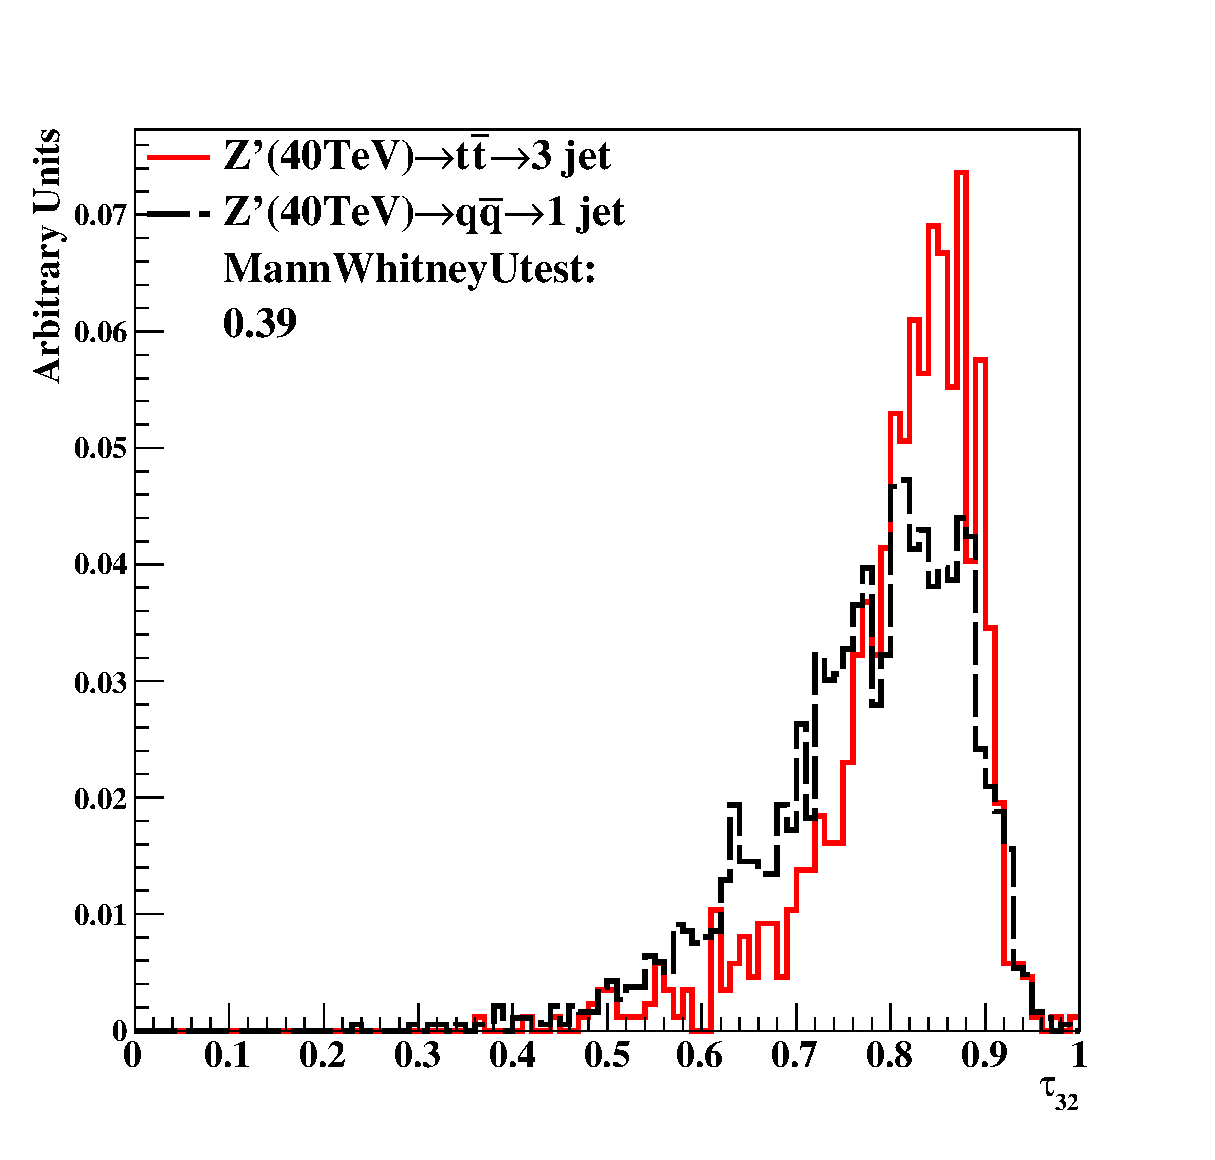
\includegraphics[width=0.43\textwidth]{figs/Dis_cluster_012_tau32_40tev_04_no_cut_Man_100.eps}
   }
   \subfigure[40TeV at 1$\times$1(cm$\times$cm) in cluster ( after cut )] {
   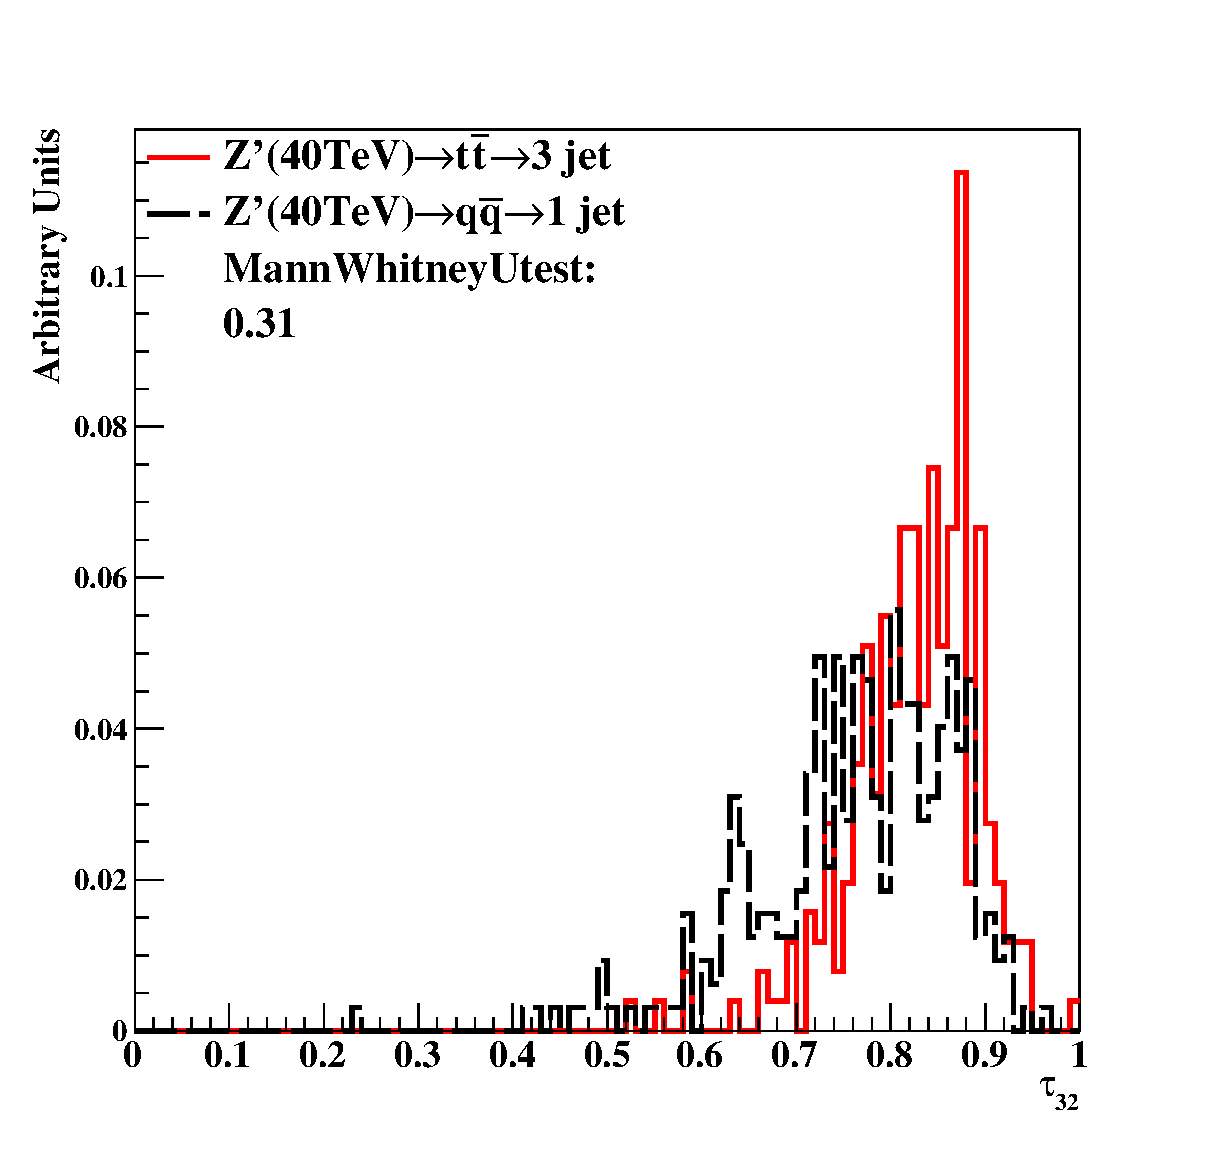
\includegraphics[width=0.43\textwidth]{figs/Dis_cluster_012_tau32_40tev_04_after_cut_Man_100.eps}
   }
\end{center}
\caption{Distributions of Mann-Whitney value U in 5, 10, 20, 40TeV energy collision for $\tau_{32}$  in different detector sizes. Cell Size in 20$\times$20, 5$\times$5, and 1$\times$1(cm$\times$cm) are shown here, and all use 100 bins here.}
\label{fig:cluster_tau21_tau32}
\end{figure}
\begin{figure}
\begin{center}
   \subfigure[40TeV at 20$\times$20(cm$\times$cm) in cluster ( no cut )] {
   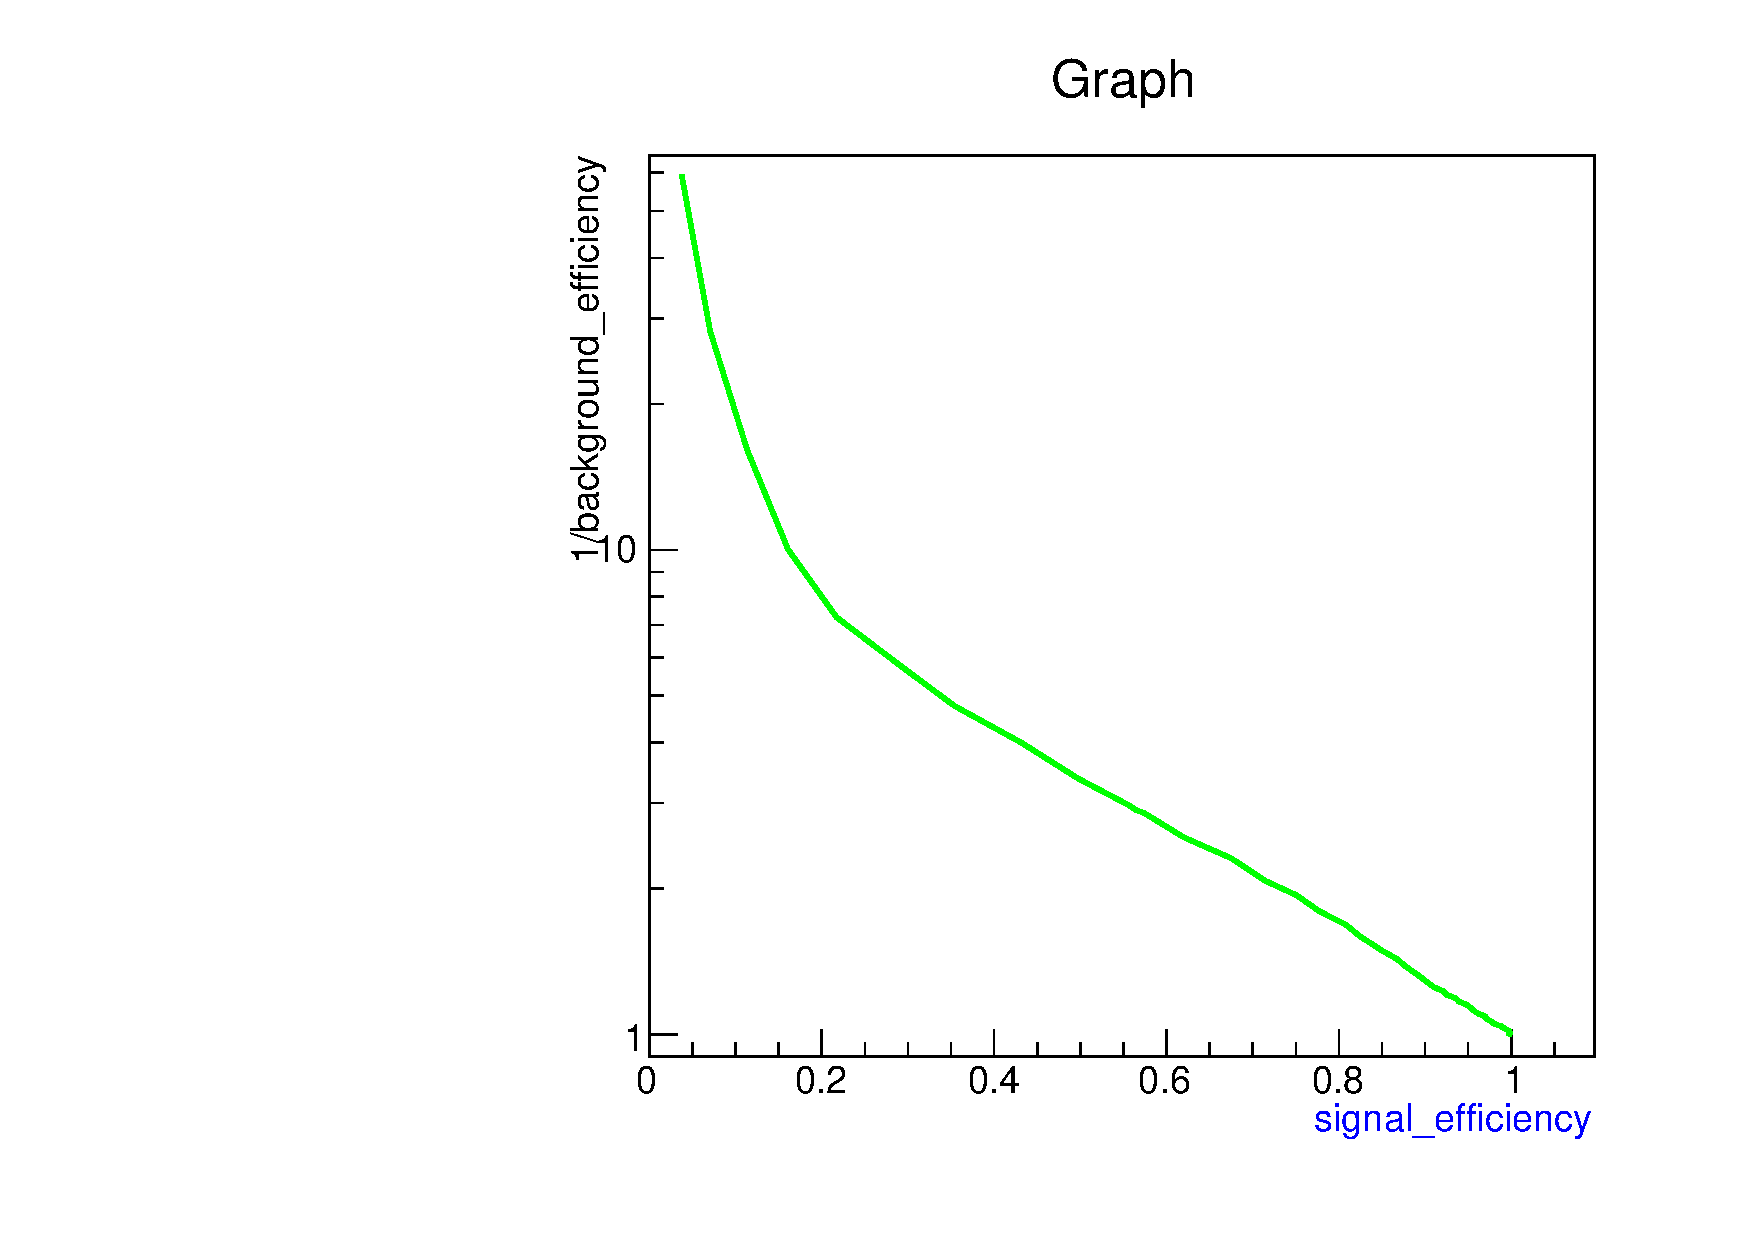
\includegraphics[width=0.43\textwidth]{figs/cluster_r010_tau32_40tev_04_eff_log_New2_no_cut.pdf}
   }
      \subfigure[40TeV at 20$\times$20(cm$\times$cm) in cluster (after cut)] {
   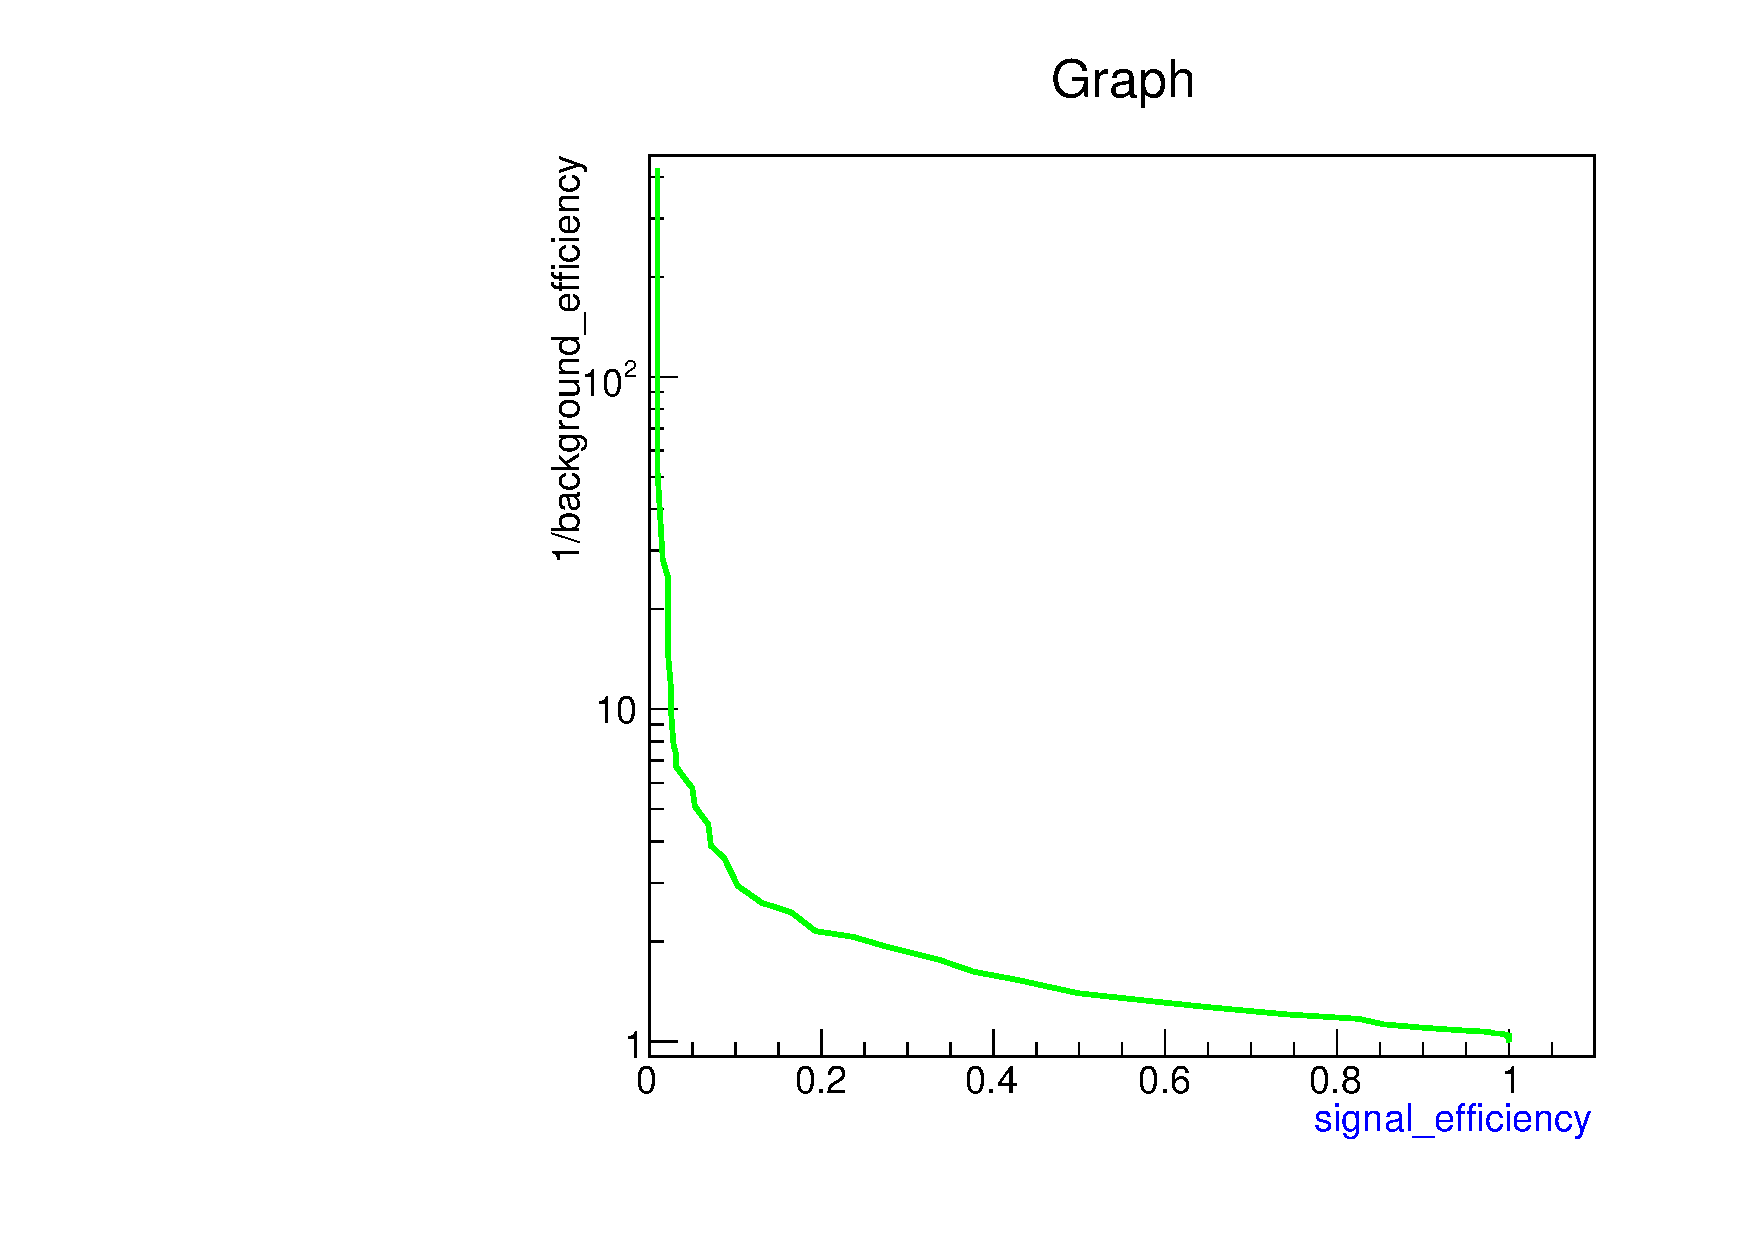
\includegraphics[width=0.43\textwidth]{figs/cluster_r010_tau32_40tev_04_eff_log_New2_50.pdf}
   }
   \subfigure[40TeV at 5$\times$5(cm$\times$cm) in cluster ( no cut )] {
   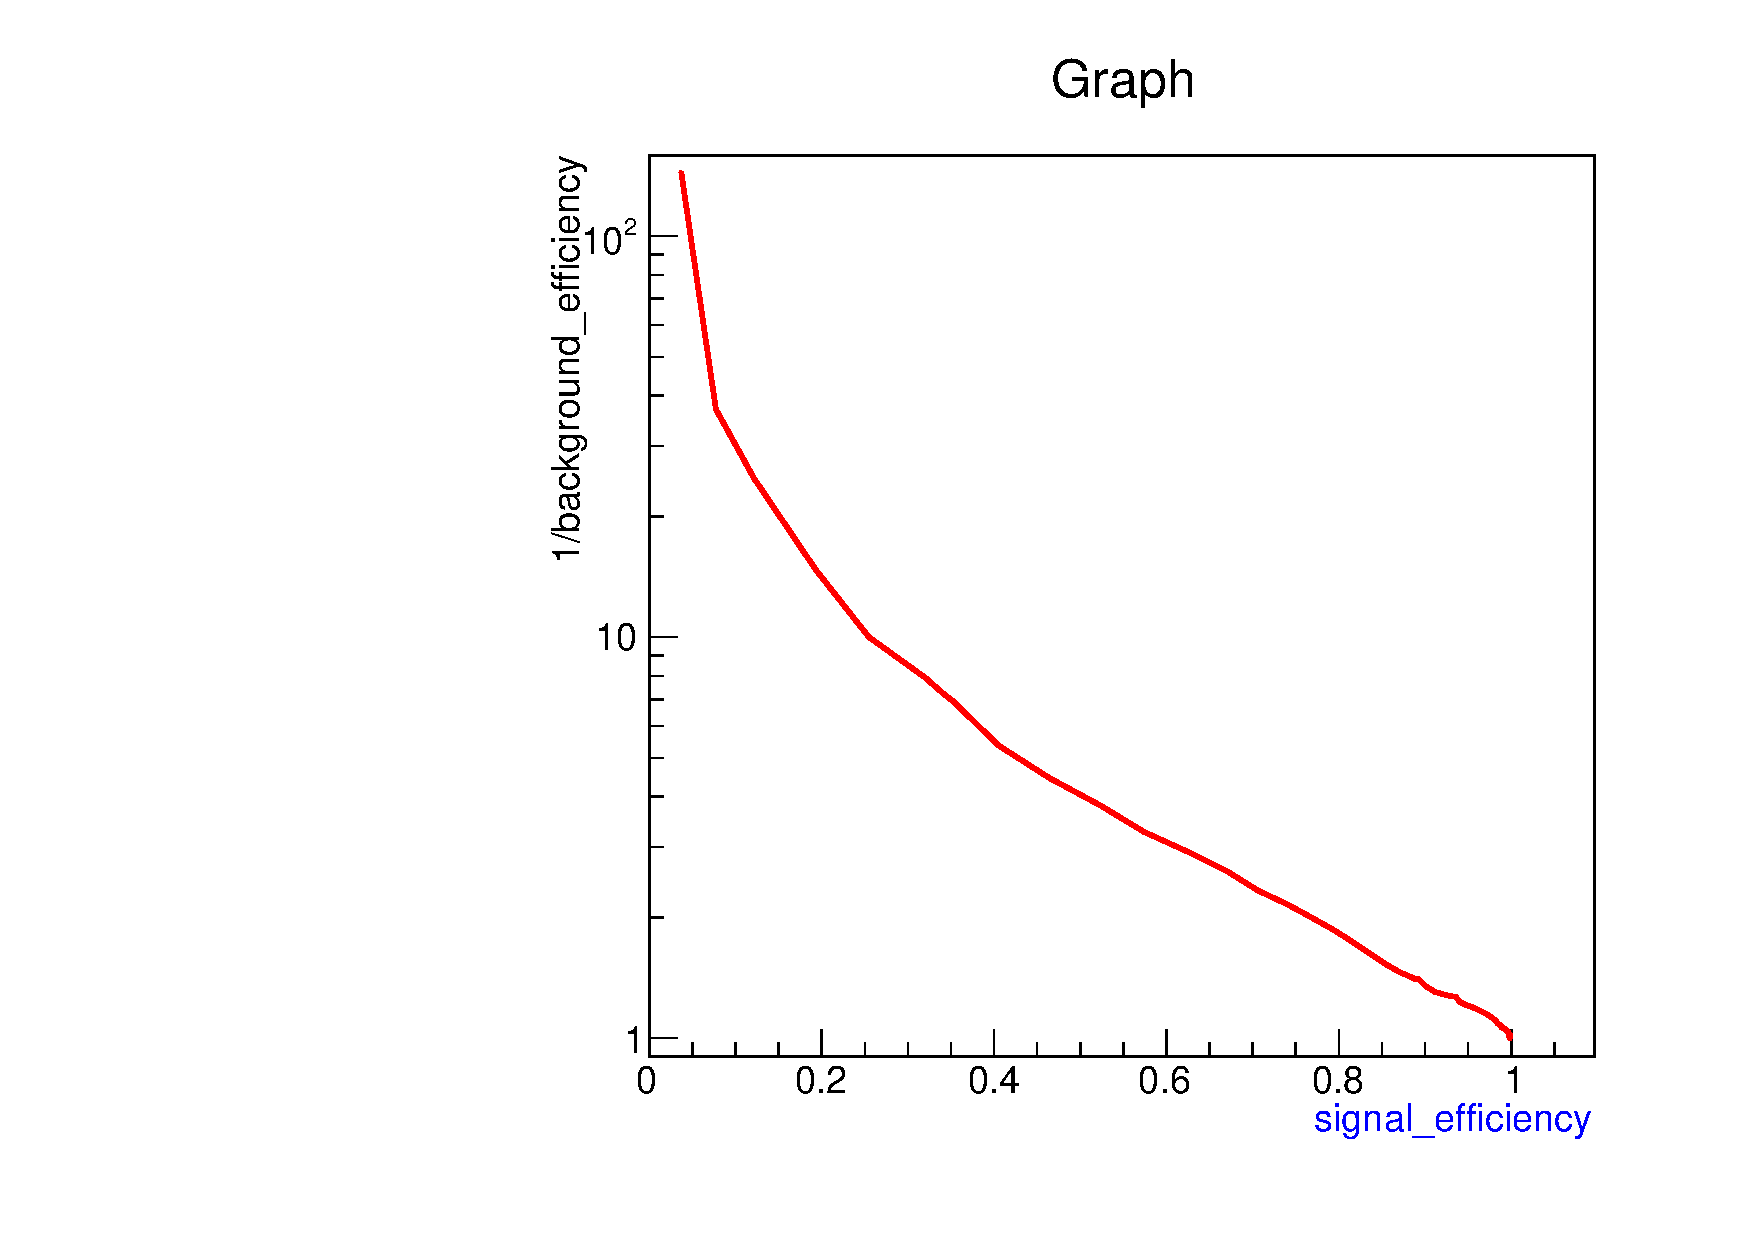
\includegraphics[width=0.43\textwidth]{figs/cluster_r009_tau32_40tev_04_eff_log_New2_no_cut.pdf}
   }
    \subfigure[40TeV at 5$\times$5(cm$\times$cm) in cluster ( after cut )] {
   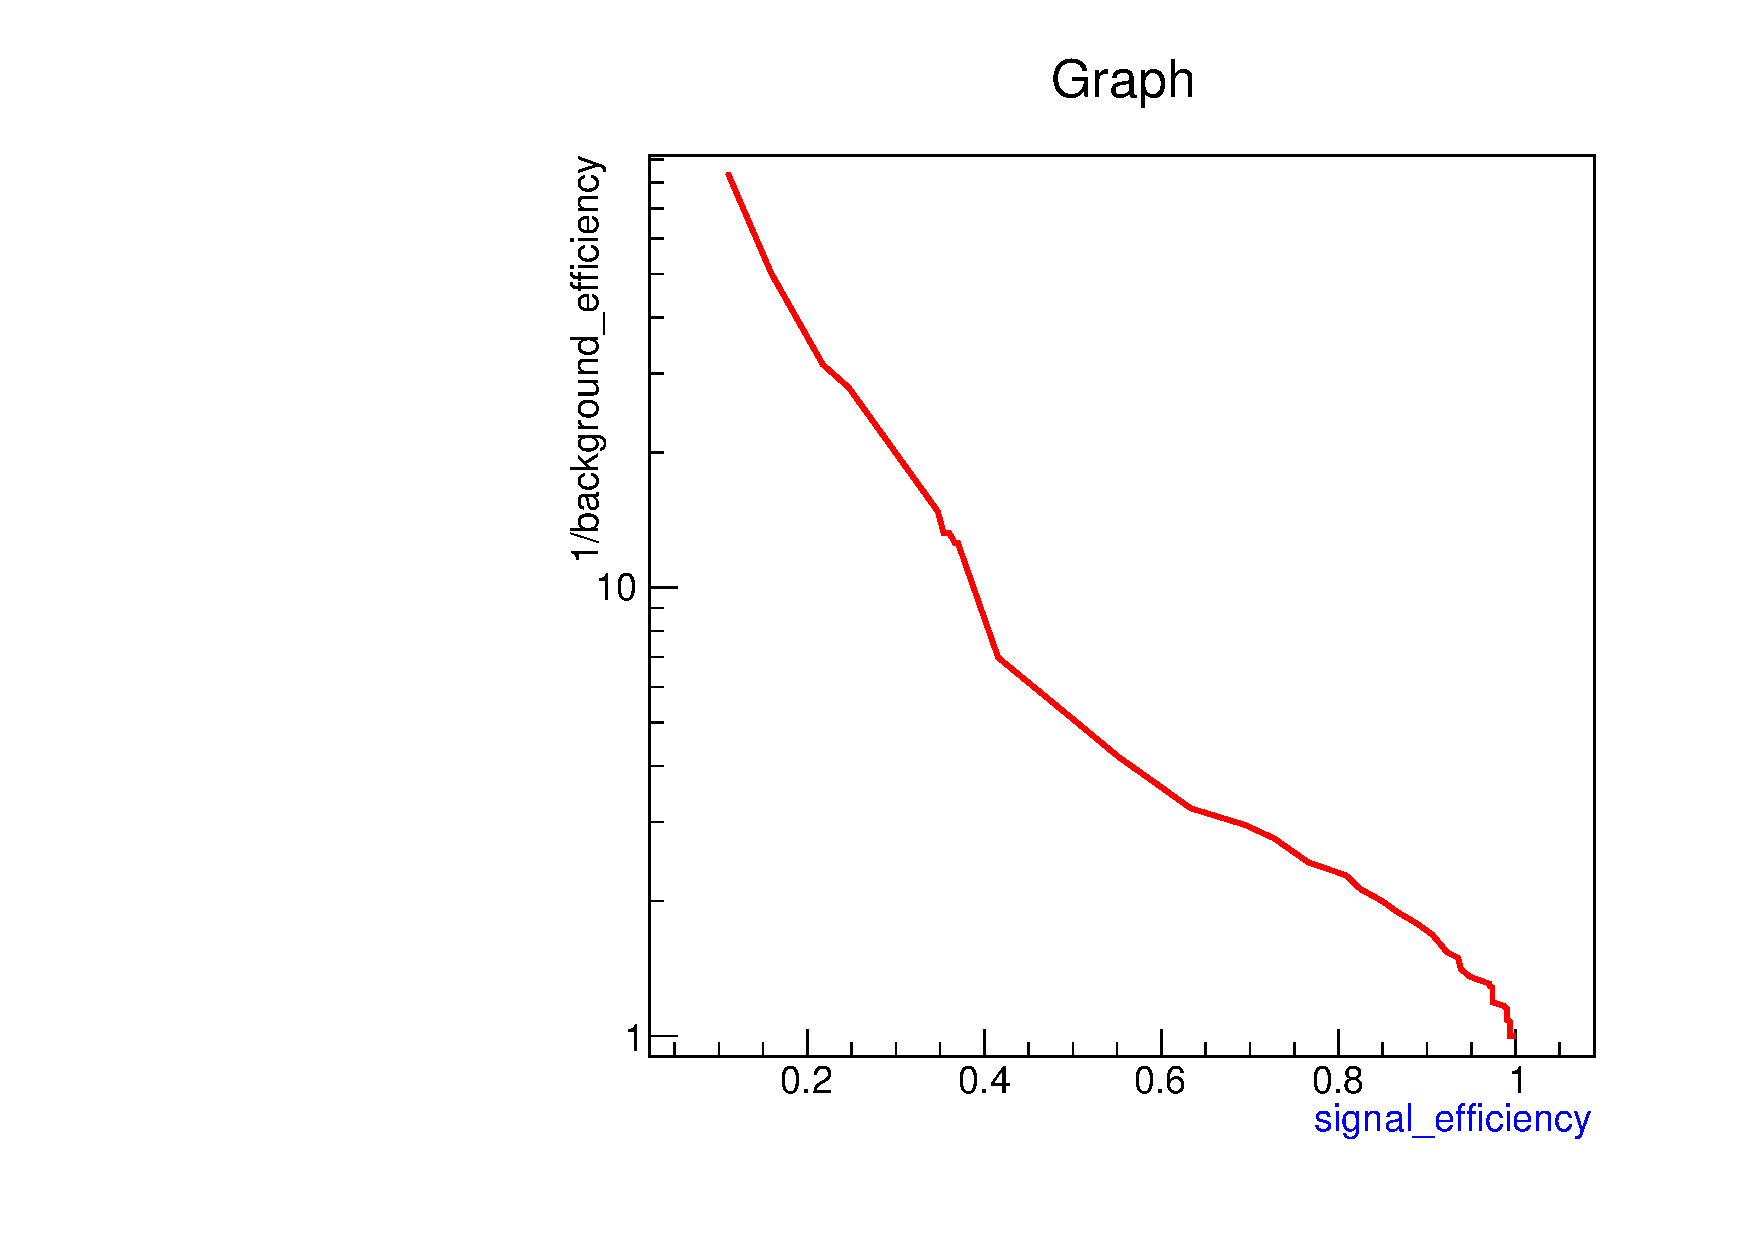
\includegraphics[width=0.43\textwidth]{figs/cluster_r009_tau32_40tev_04_eff_log_New2_50.pdf}
   }
   \subfigure[40TeV at 1$\times$1(cm$\times$cm) in cluster ( no cut )] {
   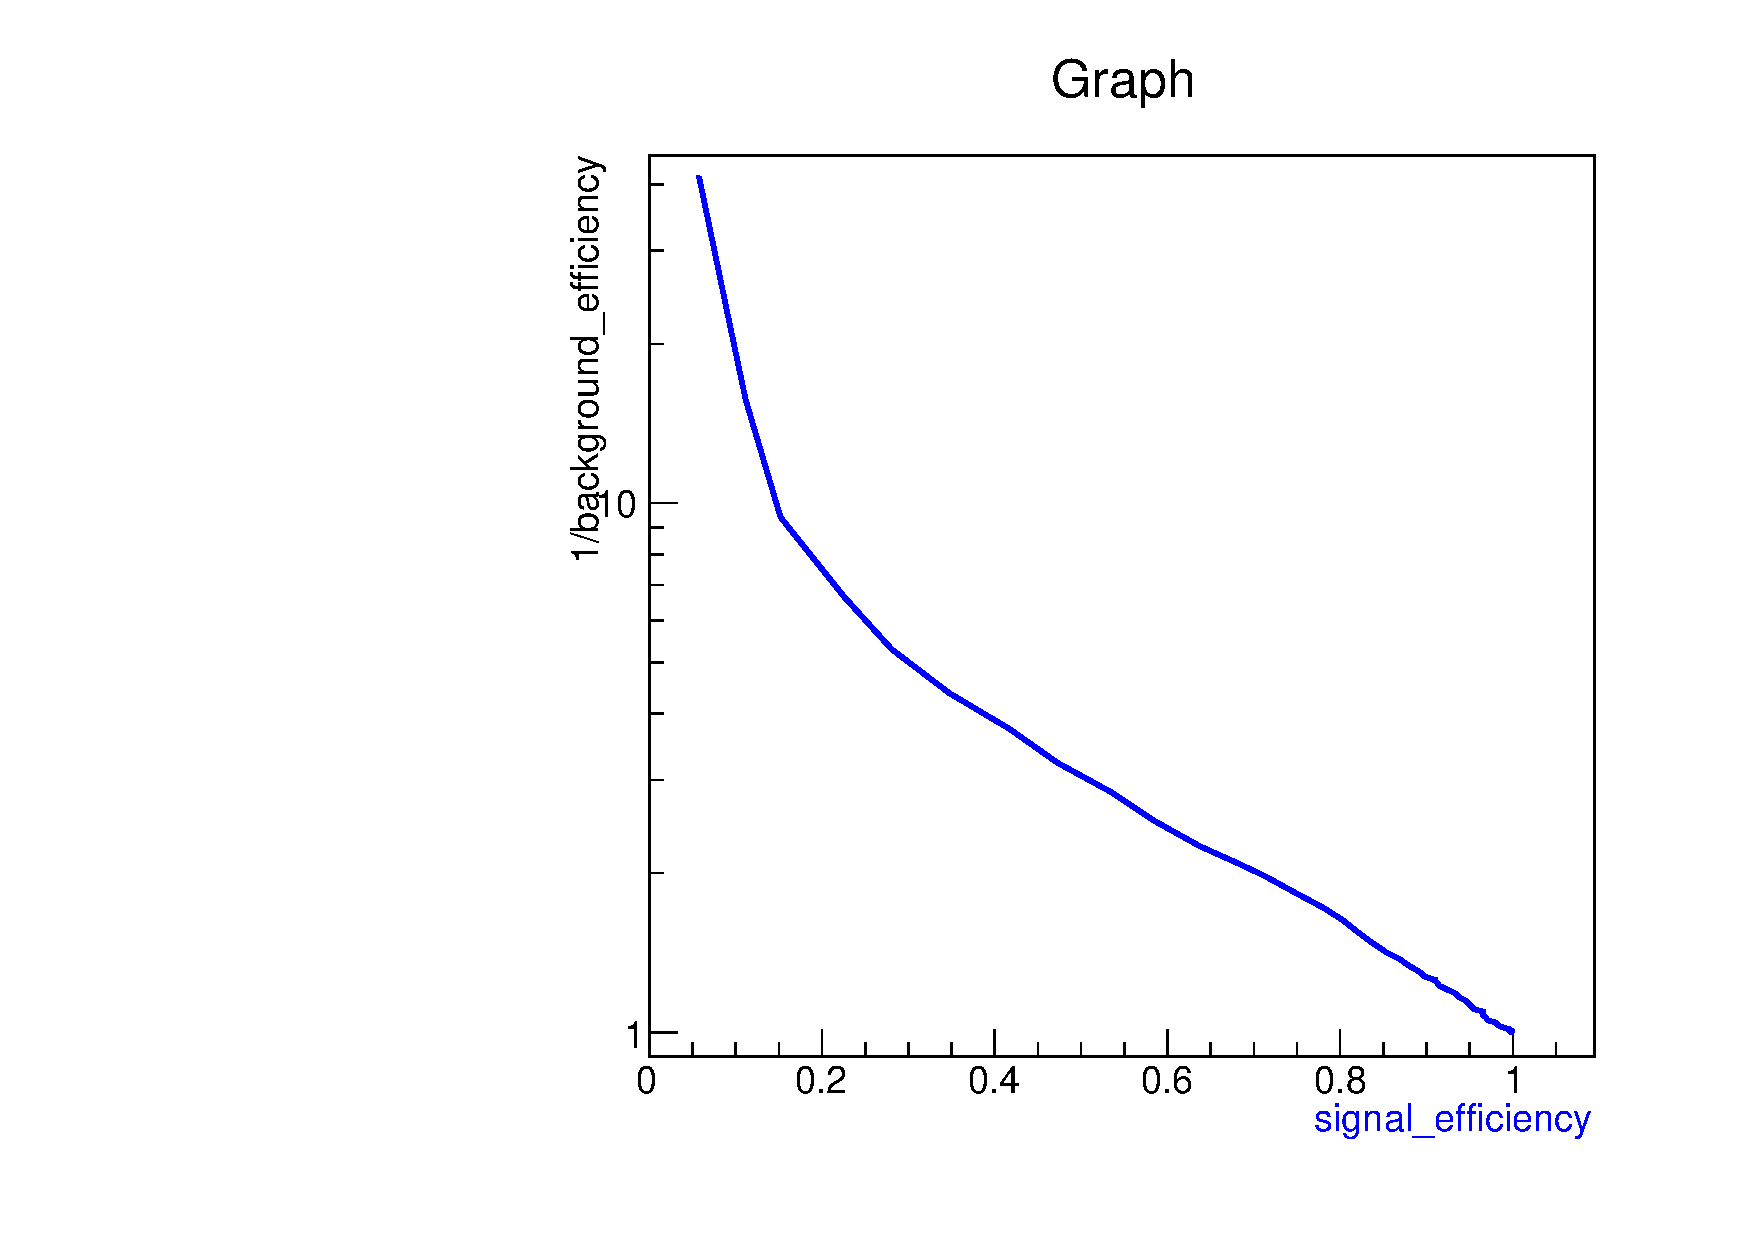
\includegraphics[width=0.43\textwidth]{figs/cluster_r012_tau32_40tev_04_eff_log_New2_no_cut.pdf}
   }
   \subfigure[40TeV at 1$\times$1(cm$\times$cm) in cluster ( after cut )] {
   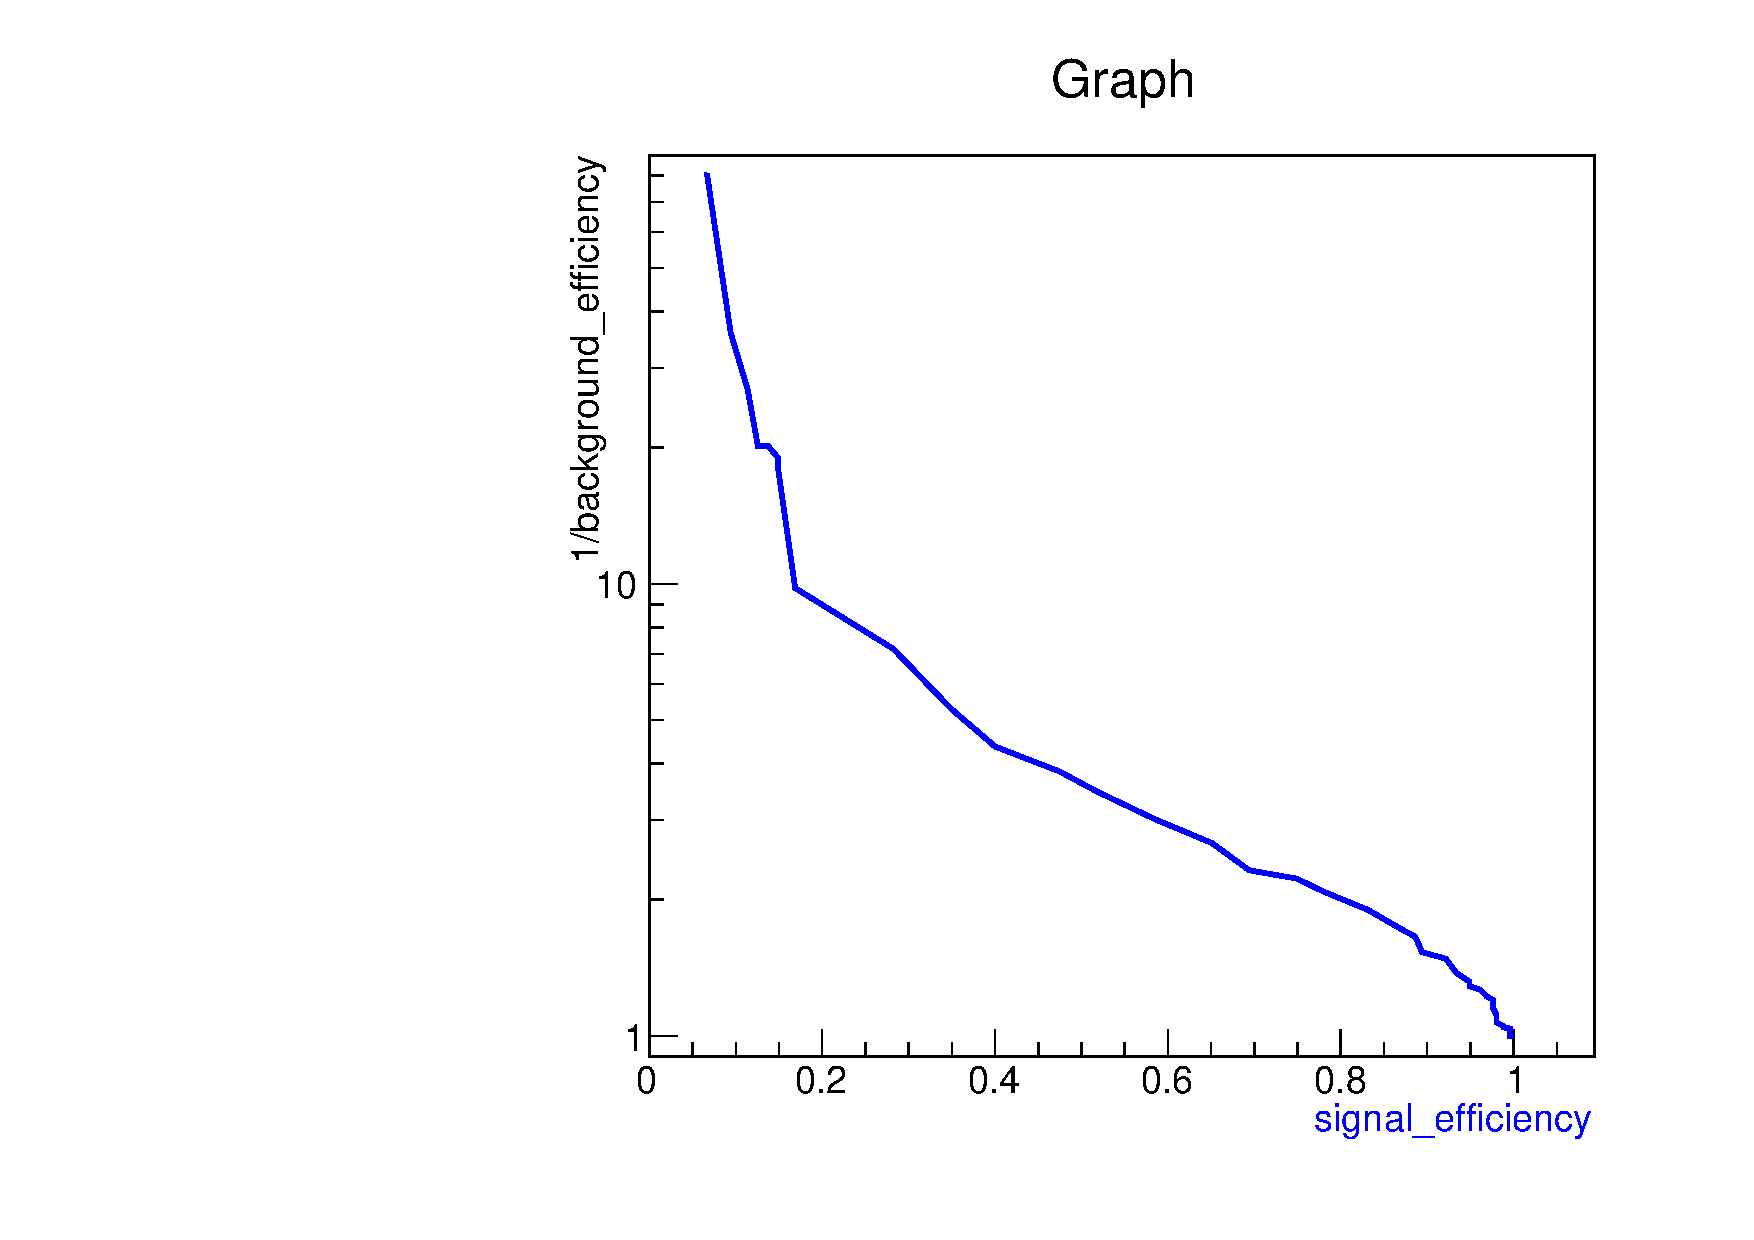
\includegraphics[width=0.43\textwidth]{figs/cluster_r012_tau32_40tev_04_eff_log_New2_50.pdf}
   }
\end{center}
\caption{Signal efficiency versus background rejection rate using $\tau_{32}$, all use 100 bins.}
\label{fig:cluster_tau21_tau32}
\end{figure}

\begin{figure}
\begin{center}
   \subfigure[5 TeV using cluster method with New2 no cut Method] {
   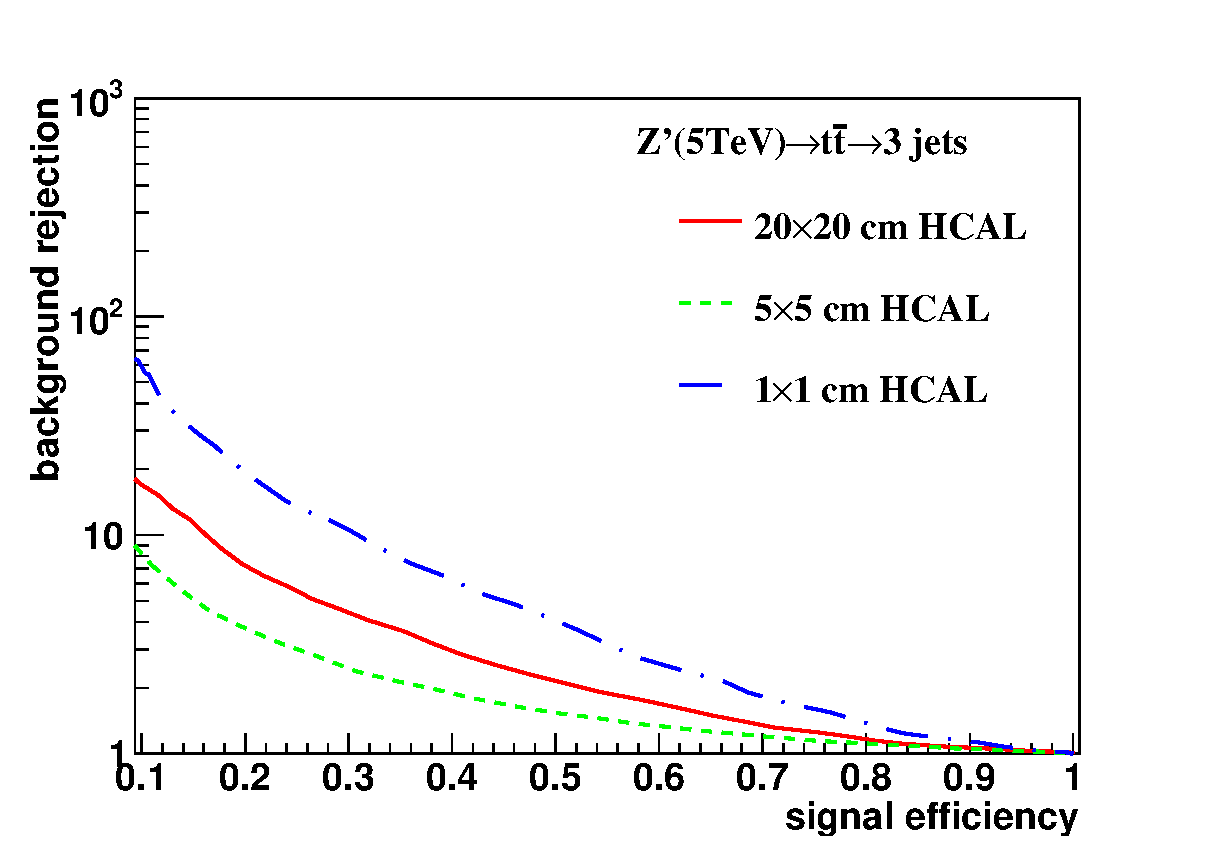
\includegraphics[width=0.43\textwidth]{figs/cluster_tau32_5tev_eff_1_New2_no_cut.eps}\hfill
   }
   \subfigure[10 TeV using cluster method with New2 no cut Method] {
   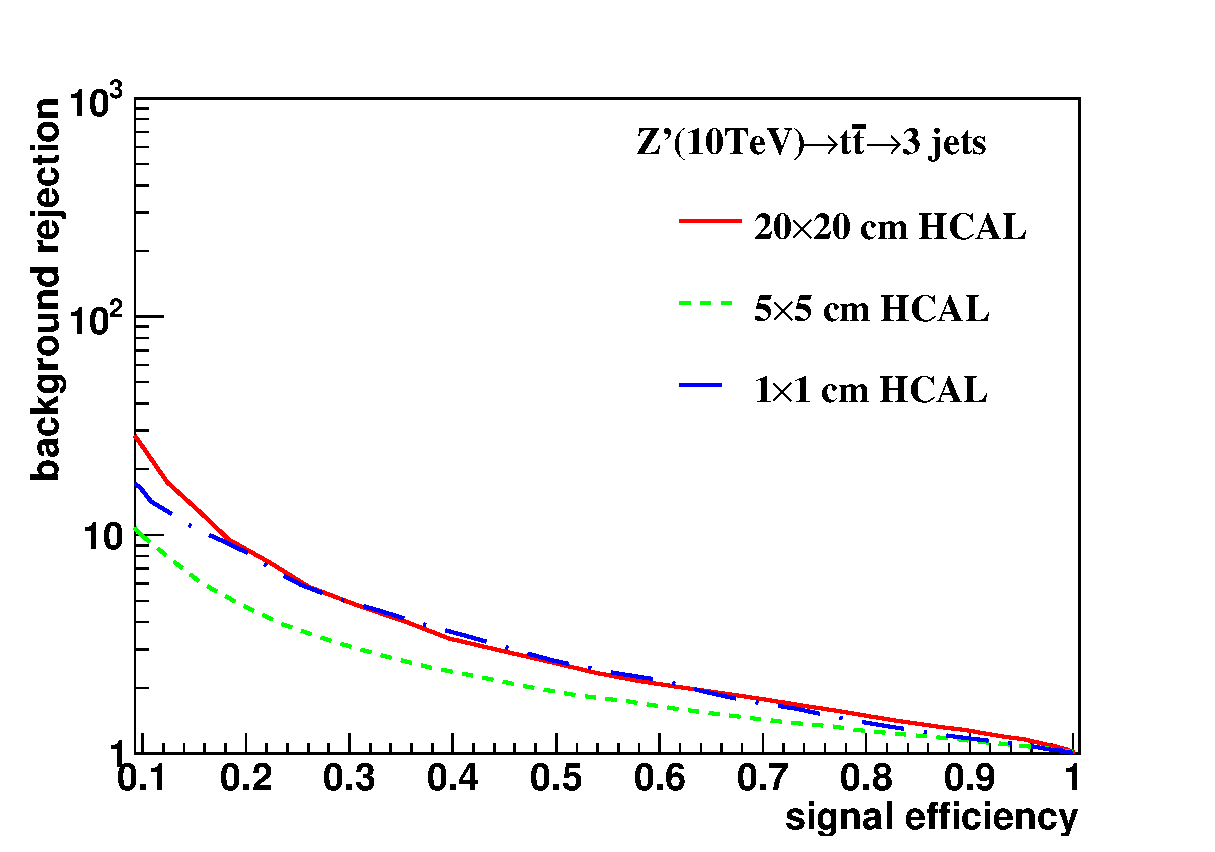
\includegraphics[width=0.43\textwidth]{figs/cluster_tau32_10tev_eff_1_New2_no_cut.eps}
   }
   \subfigure[20 TeV using cluster method with New2 no cut Method] {
   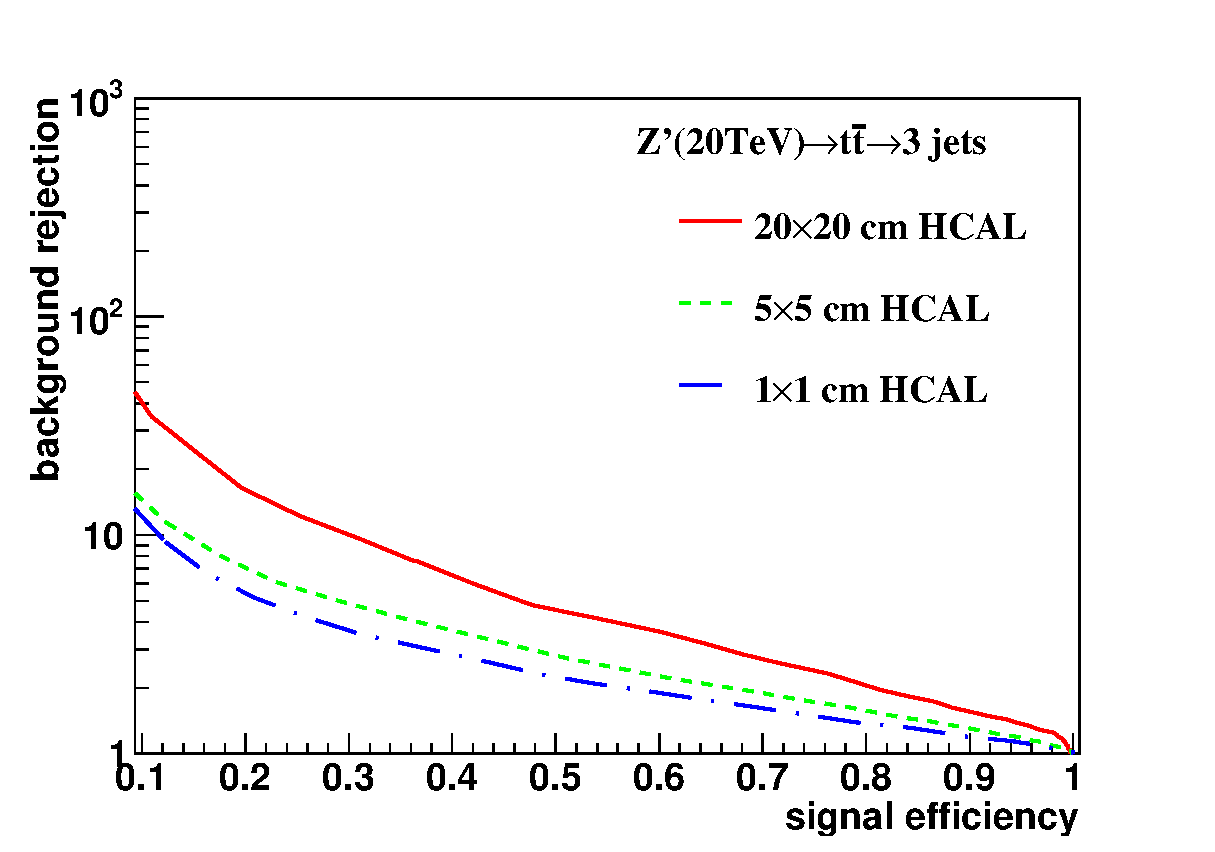
\includegraphics[width=0.43\textwidth]{figs/cluster_tau32_20tev_eff_1_New2_no_cut.eps}
   }
   \subfigure[40 TeV using cluster method with New2 no cut Method] {
   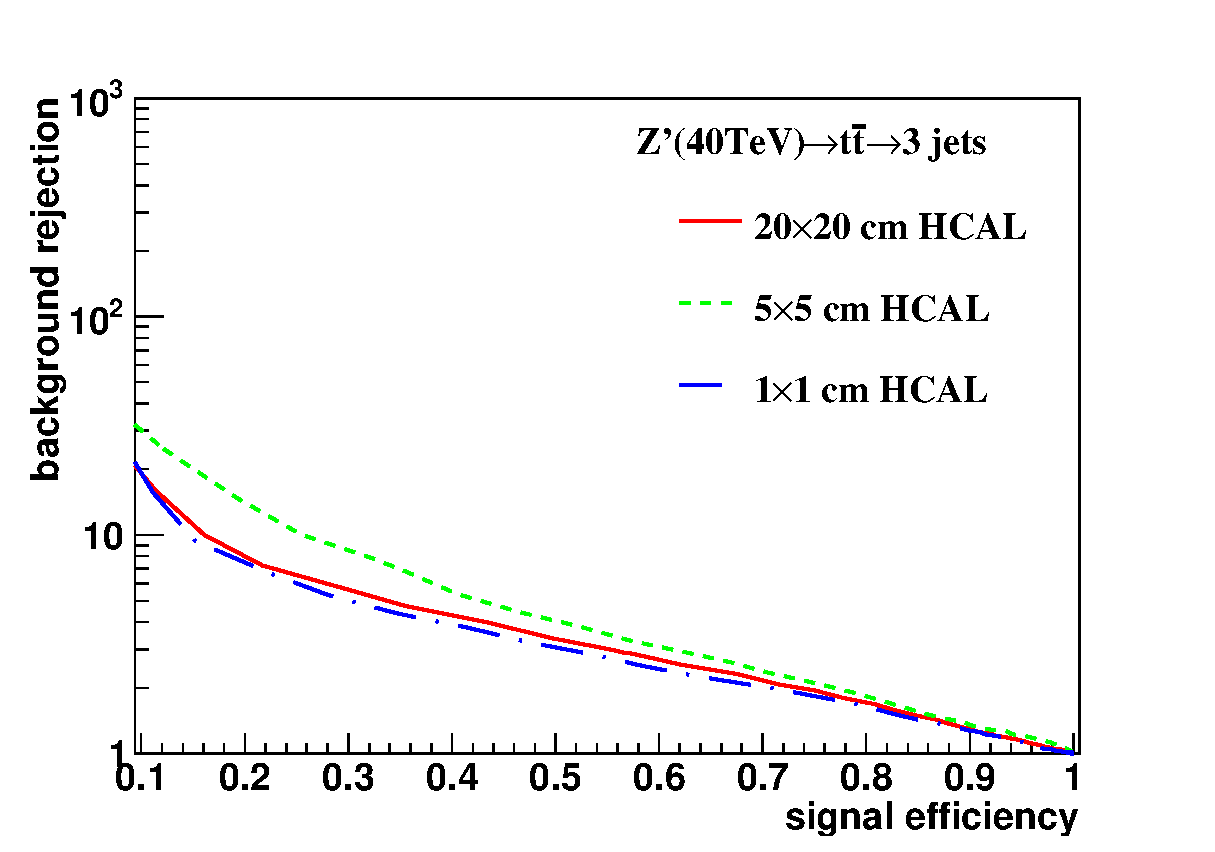
\includegraphics[width=0.43\textwidth]{figs/cluster_tau32_40tev_eff_1_New2_no_cut.eps}
   }
\end{center}
\caption{Signal efficiency versus background rejection rate using $\tau_{32}$ .The energies of collision at (a)5, (b)10, (c)20, (d)40TeV are shown here. In each picture, the three ROC curves correspond to different detector sizes.}
\label{fig:cluster_tau32}
\end{figure}

\begin{figure}
\begin{center}
   \subfigure[5 TeV using cluster method with New2 after cut Method] {
   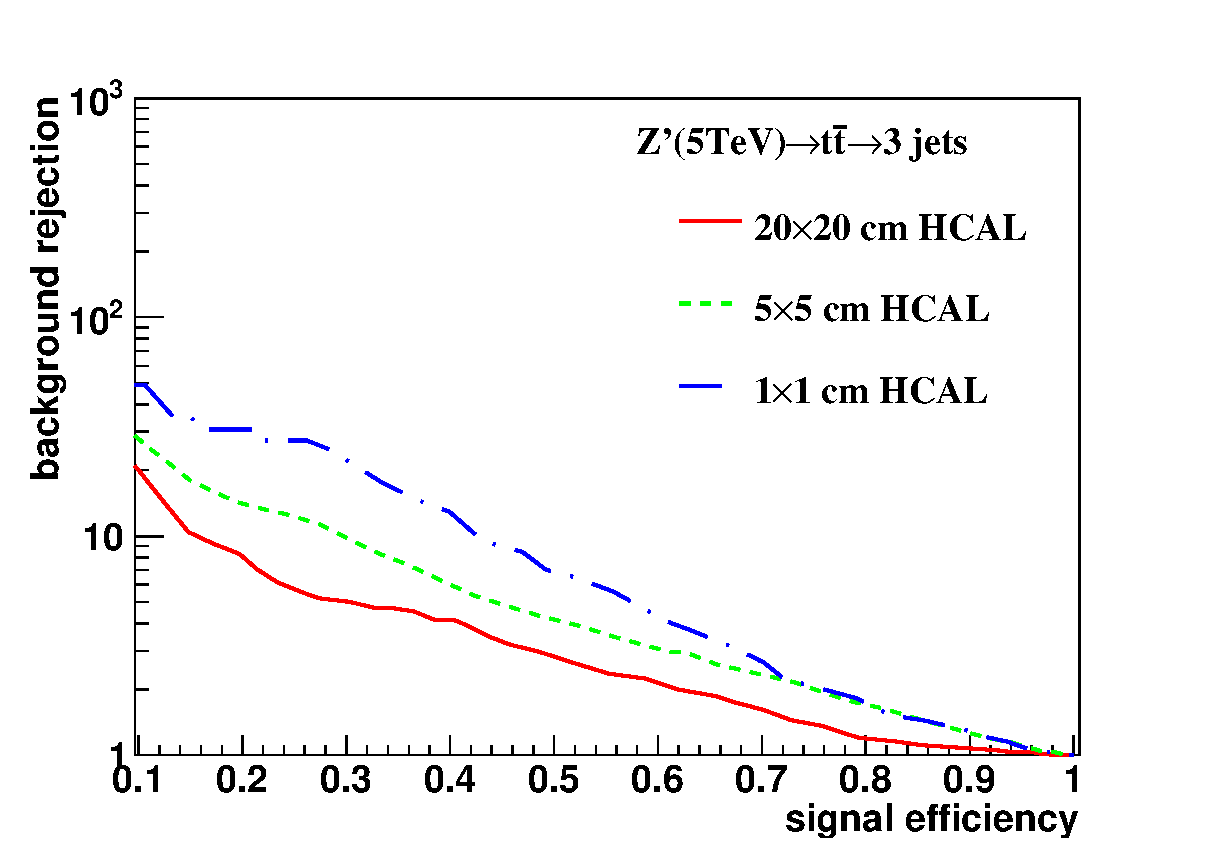
\includegraphics[width=0.43\textwidth]{figs/cluster_tau32_5tev_eff_1_New2_after_cut.eps}\hfill
   }
   \subfigure[10 TeV using cluster method with New2 after cut Method] {
   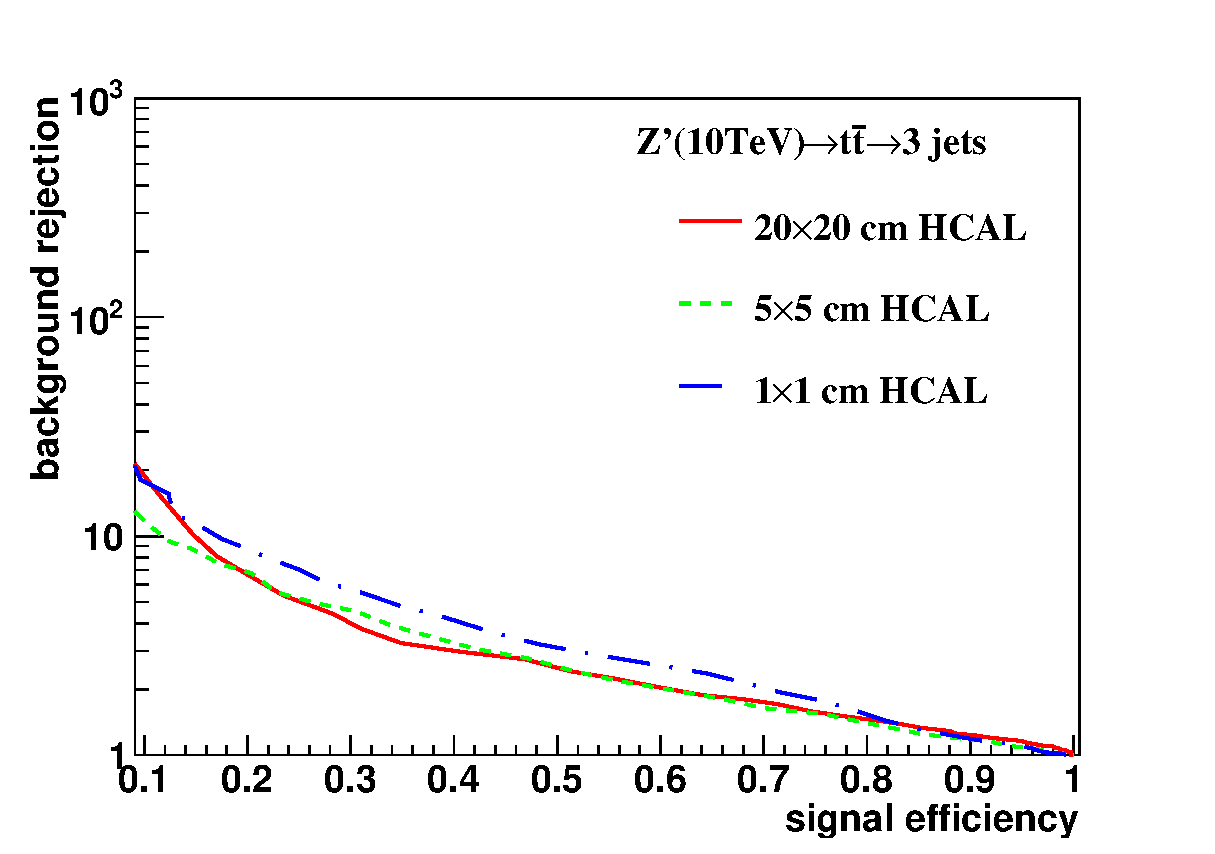
\includegraphics[width=0.43\textwidth]{figs/cluster_tau32_10tev_eff_1_New2_after_cut.eps}
   }
   \subfigure[20 TeV using cluster method with New2 after cut Method] {
   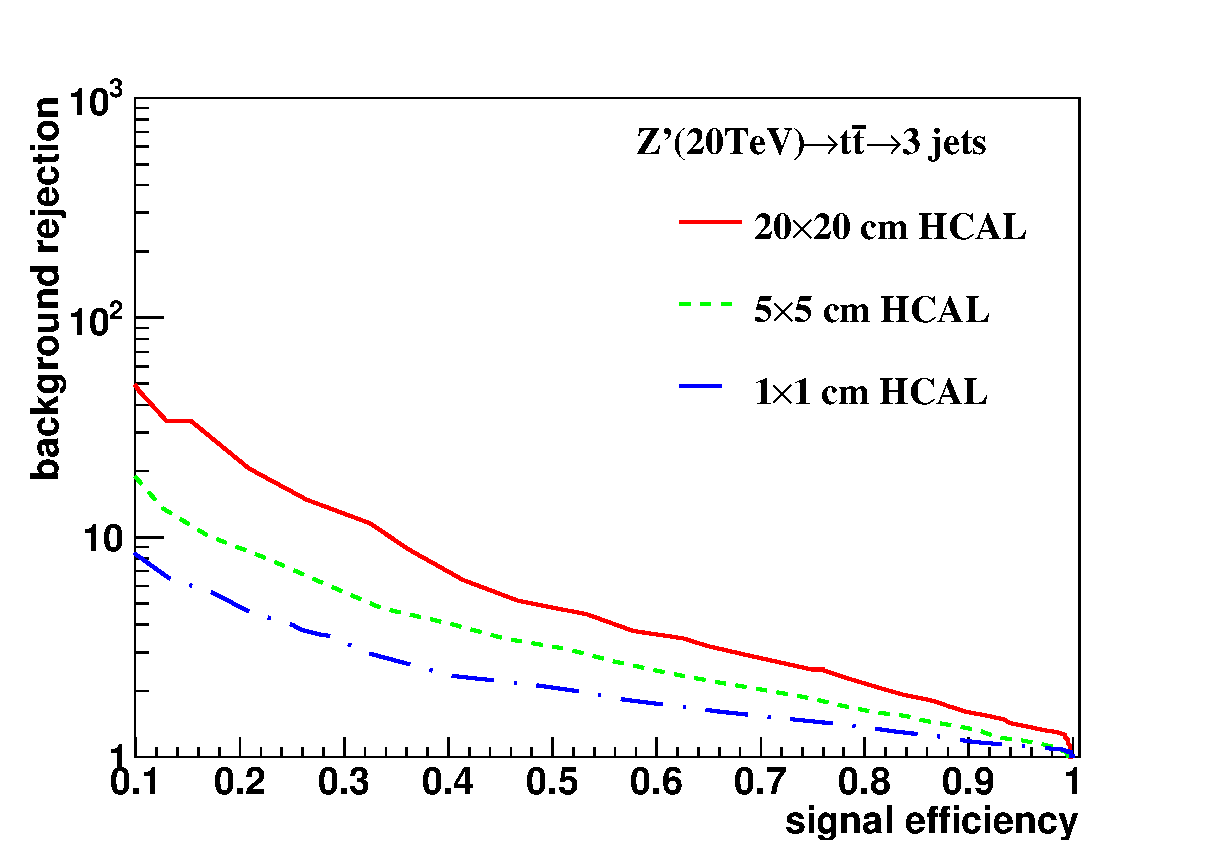
\includegraphics[width=0.43\textwidth]{figs/cluster_tau32_20tev_eff_1_New2_after_cut.eps}
   }
   \subfigure[40 TeV using cluster method with New2 after cut Method] {
   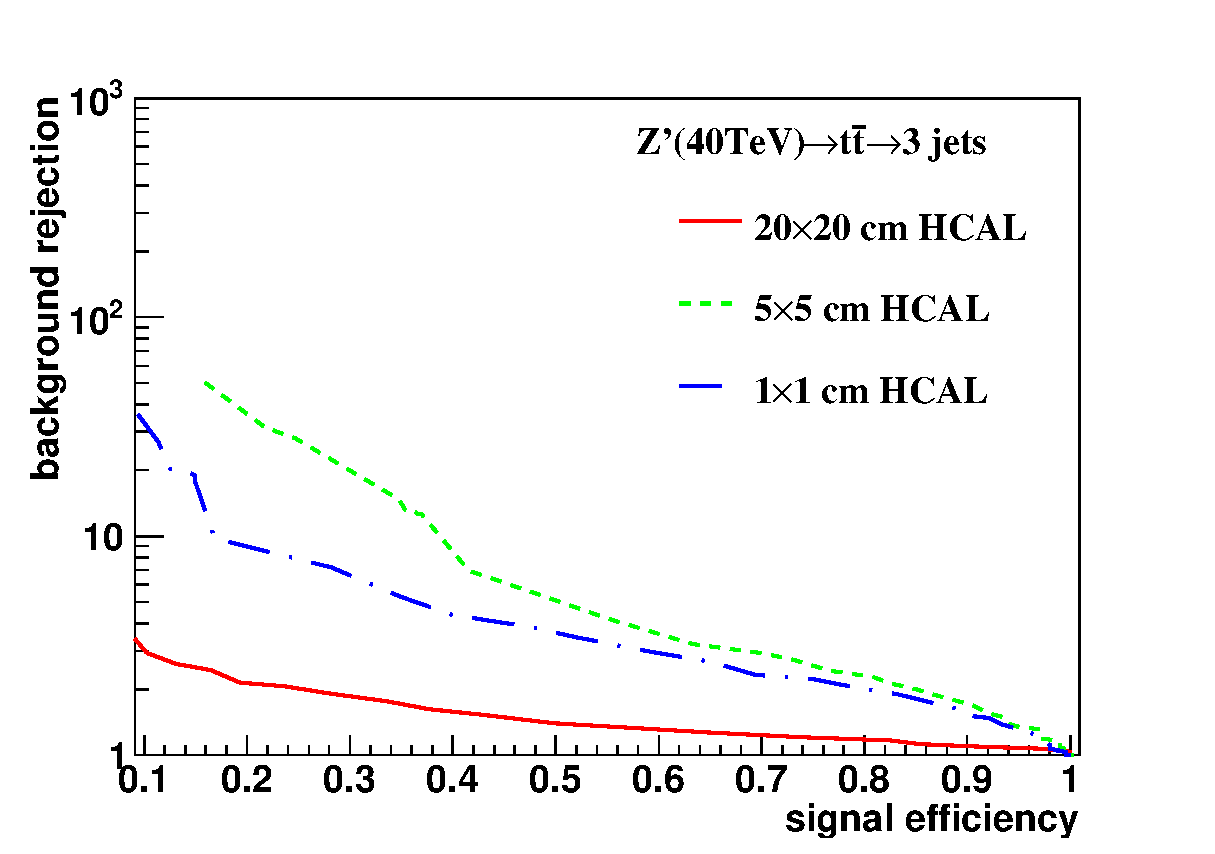
\includegraphics[width=0.43\textwidth]{figs/cluster_tau32_40tev_eff_1_New2_after_cut.eps}
   }
\end{center}
\caption{Signal efficiency versus background rejection rate using $\tau_{32}$ .The energies of collision at (a)5, (b)10, (c)20, (d)40TeV are shown here. In each picture, the three ROC curves correspond to different detector sizes.}
\label{fig:cluster_tau32}
\end{figure}

\end{document}




